\problemname{Investigator of Crashes
}

\begin{center}
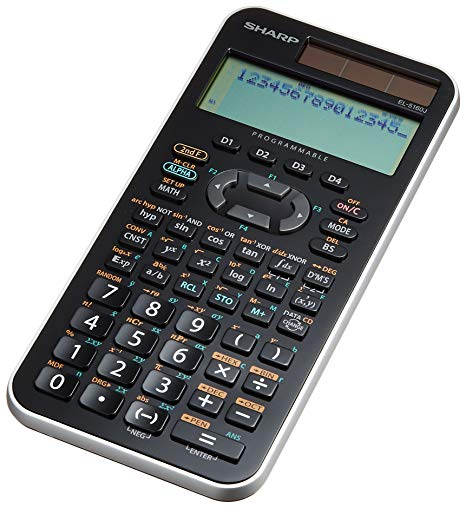
\includegraphics[scale=0.2]{calculator.jpg}
\end{center}

You have been hired as an Investigator of Crashes in Programmable Calculators.
The calculator software you are investigating allows the definition of fixed point functions.
Each such function consists of statements of the form \texttt{+x}, \texttt{-x}, \texttt{*x}, or \texttt{/x}, where \texttt{x} denotes some non-negative integer, except for division, where \texttt{x} is positive. Each operator appears exactly once, in some order.

The function takes a non-negative integer as input, and repeatedly (in a potentially endless loop) applies the specified operations to it in order, by adding, subtracting, multiplying with, or dividing by the given integer. Division is implemented as integer division and rounds down.

The software supports non-negative integers of arbitrary size, but cannot handle negative integers---if any operation would result in a negative value, the calculator crashes.
If no crash occurs, the function will either run forever or until a fixed point is reached (that is, when applying the sequence of operations does not change the value), at which point it will stop.

Thus, when a non-negative integer is input to the function, there are exactly three possible outcomes: (1) it stops at some fixed point, (2) it crashes due to a negative number, or (3) it runs forever.

Consider the function \texttt{-1 /2 +3 *1}. An input value of $8$ produces the sequence
$8 \mapsto 6 \mapsto 5 \mapsto 5$, while an input of $1$ produces $ 1\mapsto 3 \mapsto 4 \mapsto 4$. So both $8$ and $1$ stop at a fixed point.
An input of $0$ will cause a crash since the first operation is to subtract 1, resulting in a negative number. There are no inputs that cause this function to run forever. However, all inputs will run forever for the function \texttt{+10 *3 /1 -0}.

You are given a list of functions. For each function, find the smallest non-negative input that will make the function stop, or state that such a number does not exist.

\section*{Input}

The first line of input contains a single integer $N$~($1 \leq N \leq 10\,000$), which is the number of functions to consider.

The next $N$ lines describe the functions. Each of these lines contains exactly 4 statements of the form \texttt{+x}, \texttt{-x}, \texttt{*x}, or \texttt{/y}, with $0\leq x\leq 10^6$ and $1 \leq y \leq 10^6$.
Each operator appears exactly once.


\section*{Output}

For each function, display the smallest non-negative input that will make each function stop. If there is no such input, display \texttt{BAD CODE} instead.
